\chapter{Introduction}
%
In recent years, two-dimensional (2D) layered materials~\cite{2dmat, LI2016322, https://doi.org/10.1002/smll.202107059} have garnered significant attention because they exhibit exciting optical~\cite{optic1, yuHighlyEfficientGatetunable2013, dengBlackPhosphorusMonolayer2014, chengElectroluminescencePhotocurrentGeneration2014}, thermal~\cite{popThermalPropertiesGraphene2012, chenThermoelectricTransportGraphene2015}, and electronic~\cite{britnellFieldEffectTunnelingTransistor2012, georgiouVerticalFieldeffectTransistor2013, yuVerticallyStackedMultiheterostructures2013,moriyaLargeCurrentModulation2014, sarkarSubthermionicTunnelFieldeffect2015} properties that change dramatically as the material is thinned down from bulk to monolayer.
%
Transition metal dichalcogenides or TMDCs are a family of materials consisting of transition metals (group 3 through 12 on the periodic table) and chalcogen atoms (Sulphur, Selenium or Tellurium) in an \ce{MX_2}-configuration, where \ce{M} is the metal atom and \ce{X_2} are the chalcogen atoms (Figure~\ref{fig:tmdc_struc}) and are a subset of the group of two-dimensional materials\cite{C7TA04268J}. The properties of TMDCs depend greatly on the amount of stacked layers and with individual layers being as thin as \SI{6.5}{\angstrom} for \ce{MoS_2}.
%
\begin{figure}
    \centering
    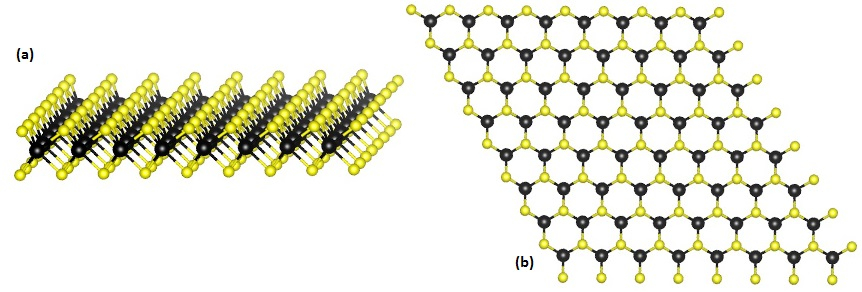
\includegraphics[width=0.7\textwidth, keepaspectratio]{resources/Figures/Monolayer_TMDC_structure.jpg}
        \caption{\textbf{a}) side-view of a TMD crystal structure. \textbf{b}) Top view of a TMD crystal structure. In both views the transition metal is black and the chalcogen atom yellow.}
    \label{fig:tmdc_struc}
\end{figure}
%
The already vast amount of tunability increases even further as one starts to stack these thin 2D building blocks into larger, potentially twisted heterostructures, exploiting Van der Waals forces that normally hold the layers in the bulk crystal~\cite{ScopusDocumentDetails, buscemaPhotocurrentGenerationTwodimensional2015, geimVanWaalsHeterostructures2013}.\\

The relative ease of manufacturing by exfoliating~\cite{bhushan2012encyclopedia,novoselovElectricFieldAtomically2004,kimLargescalePatternGrowth2009,deanBoronNitrideSubstrates2010a} to monolayer and then stamping~\cite{frisendaRecentProgressAssembly2018,castellanos-gomezDeterministicTransferTwodimensional2014} these monolayers to form precisely engineered heterostructures it is possibly to study their potential applications across diverse fields, including power electronics and solar cells~\cite{gongTwoStepGrowthTwoDimensional2015,liEpitaxialGrowthMonolayer2015,duanLateralEpitaxialGrowth2014,gongVerticalInplaneHeterostructures2014,hongUltrafastChargeTransfer2014}, single-photon emitters~\cite{koperskiSinglePhotonEmitters2015, rosenbergerQuantumCalligraphyWriting2019, pengCreationSinglePhotonEmitters2020}, and biosensors~\cite{loanGrapheneMoS2Heterostructures2014}, underscore the significance of studying these materials.\\
%\textcolor{red}{what do you mean by ease ... is the stamping right? perhaps you could explain it here...thanks to the weak vdW we can easily exfoliate them and stack many different materials one on top of each other creating a wide variety of heterostructures each of them with different .}\\

This research is motivated by the need to understand these fascinating materials and the dynamic interplay between tunable physical properties, such as strain, twist angle (referring to the relative rotation of individual layers in the heterostructure), and material combinations. The manipulation of these properties not only holds promise for novel applications across various fields but also leads to intriguing physical phenomena arising from the rotation of layers in these heterostructures.

For instance, superconductivity in magic angle graphene~\cite{caoUnconventionalSuperconductivityMagicangle2018} and single-photon emission at \SI{150}{\kelvin} in monolayer $WSe_2$~\cite{partoDefectStrainEngineering2021}.\\
%\textcolor{red}{...add concrete examples and explain the physics underneath of this configuration. Some examples are: unconventional superconductivity in twisted bilayer graphene; you could also add examples that exhibit SPE, etc...Here also add Refs.}\\

To achieve this goal, we require advanced techniques capable of pinpointing nanometer-scale features, enabling correlations between spatial atomic arrangements and features such as potential fields. Therefore, this study employs scanning transmission electron microscopy (STEM) in combination with a state-of-the-art, high-speed, and high dynamic range direct electron detector to collect precise and localised information. In particular, the electron microscope pixelated array detector (EMPAD) will be used to capture the diffraction data from small areas of the heterostructure crystal lattice. By scanning the sample with a finely localised electron probe in a rasterised pattern, we generate comprehensive four-dimensional (4D) datasets. These 4D datasets enable the mapping of strain, electrical properties, and potential fields with micrometre and nanometre-level precision.\\

To facilitate this research, I developed and integrated a novel centre-of-mass (COM) analysis approach into an existing dataset exploration framework. This integration streamlines experimentation during electron microscope data acquisition and subsequent data analysis. Using this new method it is possible to map momentum transfer within a moiré unit cell to gain information on interaction between the electron probe and the heterostructure. An existing method is applied to map the strain in a moiré heterostructure.

The report begins with a presentation of relevant theory on electron microscopy and crystallography (Chapter \ref{sec:theory}). We then delve into the fabrication of moir\'e heterostructures (Chapter \ref{sec:methods}) and the capabilities of the EMPAD sensor for heterostrain and COM analysis (Chapters \ref{sec:heterostrain} and \ref{sec:COM}, respectively). Finally, we discuss conclusions and future possibilities in Chapter \ref{sec:outlook}.

